\documentclass[10pt]{article}
\usepackage{icmlko}

\icmlmeta{IP 파운데이션 월드모델}{186}{안 틀리는 축은 모두가 같은 방향인 축이었다}{노트 185가 ``공유 축은 매끈하고 긁어온 축은 덩어리져 있다''로 닫았다. 재 보니 반대였고, 달력이 그 설명을 통째로 깬다 --- 대신 두 메커니즘이 남는다}

\begin{document}

\twocolumn[
\icmlheader

\begin{abstract}
노트 185가 ``트리의 우위는 긁어온 열에서만 산다''를 확정하면서 까닭을
``공유 축은 매끈하고 긁어온 축은 덩어리져 있다''로 적었다. \textbf{재 보니
반대다} --- 공유 축의 고유값 비율 중앙이 0.065 이고 긁어온 축이 0.118 이며
($p{=}0.026$) 트리가 제일 크게 이기는 위키 · 검색이 \emph{제일 매끈하다}
(0.60). 그래도 매끈함으로 가른 판은 예측대로 나왔다 --- 매끈한 열만
$+$0.249($t{=}7.7$), 덩어리 열만 $+$0.019($t{=}0.8$). \textbf{그런데
달력이 그 설명을 깬다} --- 달력은 덩어리인데(고유율 0.003$\sim$0.092)
트리가 $+$0.140($t{=}5.6$)로 크게 이기고 \textbf{능형은 $-$0.024 로 우연보다
못하다}. 매끈함이 원인이 아니다. 갈라서 둘이 나왔다. ① \textbf{부호
이질성} --- 위키 무리는 도메인 사이 부호 일관성이 \textbf{0.542}(동전)이고,
도메인별 $|r|$ 평균이 0.121 인데 부호를 살린 평균은 0.048 이다.
\textbf{60\%가 상쇄된다.} 풀링 선형은 계수 하나를 쓰므로 상쇄를 그대로
먹고, 트리는 도메인으로 먼저 쪼갠다. ② \textbf{비단조 · 상호작용} ---
달력은 주기 열이라 단조 계수로 표현할 수 없다. 능형이 음수인 것이 그
증거다. \textbf{공유 축 다섯은 둘 다 없다} --- 일관성 0.800,
\texttt{target\_breadth} 가 여덟 도메인 \textbf{8/8}, \texttt{media\_push}
가 \textbf{5/5}, 부호 살린 평균 0.229 로 상쇄가 거의 없다. 그래서 선형이
대등하다. 마지막으로 뜻밖의 수렴 하나. \textbf{부호 일관성이 제일 낮은 둘
(진입 장벽 0.57 · 장소 노출 0.57)이 정확히 노트 172가 ``지렛대로 틀린다''고
한 둘이고, 1위와 3위(타깃 폭 1.00 · 굿즈 규모 0.86)가 ``안 틀린다''고 한
둘이다.} 전혀 다른 통계인데 같은 순서를 준다.
\end{abstract}
]

\begin{figure*}[t]
\centering
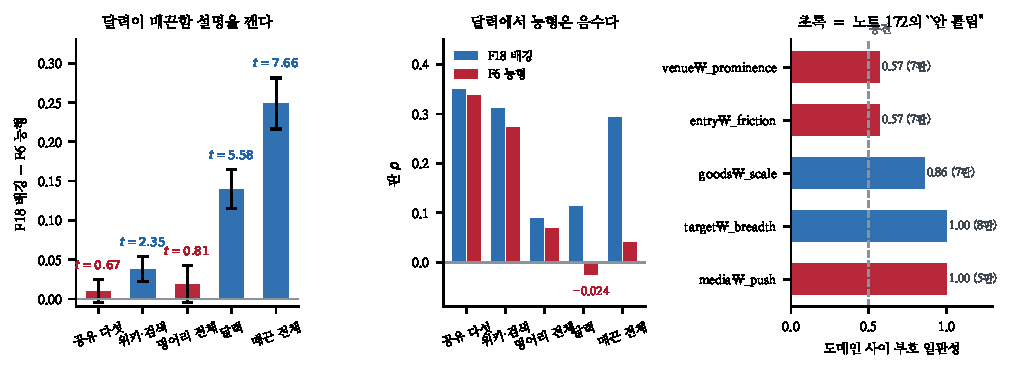
\includegraphics[width=\textwidth]{figs/mono.pdf}
\caption{왼쪽 --- 달력이 매끈함 설명을 깬다. 가운데 --- 달력에서 능형은
음수다. 오른쪽 --- 초록이 노트 172의 ``안 틀림''.}
\end{figure*}

\section{매끈함 읽기가 반대였다}

\begin{table}[t]
\centering\tsize
\caption{열의 고유값 비율(고유값 수 $\div$ 관측 행). 클수록 매끈.}
\begin{tabular}{lrr}
\toprule
& 열 수 & 중앙 \\
\midrule
\textbf{공유 축} & 44 & \textbf{0.065} \\
\textbf{긁어온 축} & 124 & \textbf{0.118} \\
\midrule
\multicolumn{3}{l}{위키 넷 0.60 · 검색 넷 0.52} \\
\multicolumn{3}{l}{진입 장벽 0.005 · 장소 노출 0.022} \\
\bottomrule
\end{tabular}
\end{table}

\claimx{\textbf{반대다}($p{=}0.026$). 노트 185가 하루 만에 쓴 읽기가
틀렸다 --- 트리가 이기는 열이 \emph{제일 매끈한} 열이다.}{\textbf{일곱 번째다}
--- 노트 157$\to$158 · 158$\to$159 · 163$\to$169 · 165$\to$166 ·
173$\to$174 · 178$\to$179, 그리고 185$\to$186. \textbf{결론 옆에 적은
``까닭''이 결론보다 훨씬 잘 틀린다.}}

\section{달력이 설명을 깬다}

\begin{table}[t]
\centering\tsize
\caption{F18 배깅 $-$ F6 능형. 짝 부트스트랩 400회.}
\begin{tabular}{lrrrl}
\toprule
열 집합 & F18 & F6 & 차 & \\
\midrule
공유 다섯 & .3499 & .3381 & $+$.010 & $t{=}0.7$ \\
위키·검색 & .3118 & .2735 & $+$.038 & $t{=}2.4$ \\
덩어리 전체 & .0889 & .0683 & $+$.019 & $t{=}0.8$ \\
\textbf{달력} & .1136 & \textbf{$-$.024} & \textbf{$+$.140} & \textbf{$t{=}5.6$} \\
매끈 전체 & .2919 & .0390 & $+$.249 & $t{=}7.7$ \\
\bottomrule
\end{tabular}
\end{table}

\claimx{\textbf{달력은 덩어리인데 트리가 크게 이긴다.} 그리고 \textbf{능형이
$-$0.024 로 우연보다 못하다} --- 단순히 못 쓰는 게 아니라 \emph{잘못
쓴다}.}{주기 열(요일 sin/cos · 월 sin/cos)이라 그렇다. 도메인마다 위상이
달라 계수 하나로는 표현이 안 되고, 억지로 맞추면 음수가 나온다.
\textbf{트리는 도메인으로 쪼갠 뒤 각자의 위상을 판다.}}

\section{두 메커니즘}

\begin{table}[t]
\centering\tsize
\caption{열 무리별. 학습 구간 도메인별 상관에서.}
\begin{tabular}{lrrrr}
\toprule
& 일관성 & $|\overline{r}|$ & $\overline{|r|}$ & 트리 우위 \\
\midrule
\textbf{공유} & \textbf{0.80} & \textbf{.229} & .229 & $+$.010 \\
검색 & 0.75 & .138 & .152 & $+$.038 \\
\textbf{위키} & \textbf{0.54} & .048 & \textbf{.121} & $+$.038 \\
\textbf{달력} & 0.65 & .034 & .057 & \textbf{$+$.140} \\
\bottomrule
\end{tabular}
\end{table}

\claimx{\textbf{① 부호 이질성.} 위키는 일관성 0.54 로 동전이고 $\overline{|r|}
{=}0.121$ 인데 $|\overline{r}|{=}0.048$ 이다 --- \textbf{60\%가 상쇄된다.}
풀링 선형은 계수 하나를 쓰므로 그 상쇄를 그대로 먹는다.}{노트 180이 위키
수준의 부호가 도메인마다 반대인 것을 재고(세계애니 $+$0.35 · 애니 $-$0.18)
노트 181이 그 까닭을 속편으로 갈랐다. \textbf{여기서 그것이 형태 선택에
어떻게 옮겨 붙는지가 나온다.}}

\claimx{\textbf{② 비단조 · 상호작용.} 달력은 상쇄가 아니라 표현력 문제다 ---
$\overline{|r|}$ 자체가 0.057 로 작은데 트리는 $+$0.114 를 낸다. 낱개
열의 단조 관계에 없는 것을 쓴다는 뜻이다.}{``12월 \emph{그리고} 주말''
같은 조합이다. \textbf{능형이 음수라는 것이 표현력 문제의 증거다} ---
상쇄면 0 으로 가지 음수로는 안 간다.}

\claimx{\textbf{공유 축은 둘 다 없다.} 일관성 0.80 · $|\overline{r}|
{=}\overline{|r|}{=}0.229$ 로 상쇄가 없고, 다섯 칸이 다 단조 양으로
설계됐다.}{그래서 선형이 대등하다($t{=}0.7$). \textbf{노트 185의 결론은
그대로 서고 그 아래 적은 까닭만 바뀐다.}}

\section{뜻밖의 수렴}

\begin{table}[t]
\centering\tsize
\caption{공유 축 다섯. 부호 일관성과 노트 172의 지렛대 판정.}
\begin{tabular}{lrrl}
\toprule
& 판 & 일관성 & 노트 172 \\
\midrule
미디어 푸시 & 5 & 1.00 & 틀림 \\
\textbf{타깃 폭} & 8 & \textbf{1.00} & \textbf{안 틀림} \\
\textbf{굿즈 규모} & 7 & \textbf{0.86} & \textbf{안 틀림} \\
\textbf{진입 장벽} & 7 & \textbf{0.57} & \textbf{틀림} \\
\textbf{장소 노출} & 7 & \textbf{0.57} & \textbf{틀림} \\
\bottomrule
\end{tabular}
\end{table}

\claimx{\textbf{일관성 꼴찌 둘이 노트 172의 ``틀린다'' 둘이다}(0.57 ·
0.57). 1위와 3위가 ``안 틀린다'' 둘이다.}{노트 172는 지렛대 충실도를 여섯
지표 $\times$ 다섯 정식화 $\times$ 아홉 도메인으로 쟀고, 여기 일관성은
학습 구간 스피어만의 부호를 세기만 한 것이다. \textbf{전혀 다른 통계인데
같은 순서를 준다.}}

\claimx{\textbf{예외가 하나 있다} --- 미디어 푸시가 일관성 1.00 인데
``틀린다''로 판정됐다. 다섯 도메인에서만 관측된다 --- 다섯이 통째로 비어
있다(노트 163).}{\textbf{덮음이 낮으면 일관성이 쉽게 1.00 이 된다.}
스피어만 $+$0.456 이라는 수렴은 다섯 점짜리이므로 세게 읽지 않는다 ---
\textbf{읽을 수 있는 것은 ``부호가 갈리는 축은 지렛대로도 틀렸다''는 방향
하나다.}}

\begin{table}[t]
\centering\tsize
\caption{남은 것.}
\begin{tabular}{ll}
\toprule
\textbf{달력} & 트리가 쓰는 조합이 무엇인지 안 봤다 \\
부호 & 도메인별 부호를 주면 선형이 따라잡나 \\
미디어 푸시 & 덮음이 낮은데 일관성 1.00 --- 믿을 값인가 \\
\bottomrule
\end{tabular}
\end{table}

두 번째 줄이 곧바로 잴 수 있고 값이 크다. 이 노트의 ① 이 맞다면 위키
열에 \emph{도메인별 부호}를 곱해 주면 능형이 트리를 따라잡아야 한다 ---
노트 180에서 그걸 해 봤고 $+$0.0018($t{=}0.6$)이었다. \textbf{안 따라잡았다.}
그러면 위키의 트리 우위도 부호 이질성만이 아니라는 뜻이고, ② 가 위키에도
있다는 쪽으로 기운다. \textbf{노트 180의 실패가 여기서 증거가 된다.}

\end{document}
